\section{Results}
\label{sec:results}

\subsection{Data Quality and Class Imbalance}

Table~\ref{tab:qc} summarises the quality-control findings. The dataset is
complete and free of missing values; the only cleaning step required was
removing exact duplicates, of which 19 were fraudulent --- a detail worth noting
because duplicate fraud rows inflate the apparent difficulty of the minority
class.

\begin{table}[h!]
\centering
\caption{Data quality report for the cleaned dataset.}
\label{tab:qc}
\begin{tabular}{p{6.5cm}p{4cm}p{4cm}}
\toprule
\textbf{Check} & \textbf{Result} & \textbf{Action} \\
\midrule
Shape (raw) & 284{,}807 $\times$ 31 & --- \\
Shape (clean) & 283{,}726 $\times$ 31 & 1{,}081 duplicates removed \\
Missing values & 0 & none required \\
Duplicate rows & 1{,}081 (1{,}062 legit / 19 fraud) & removed \\
Negative amounts & 0 & none \\
Zero amounts & 1{,}808 across the full cleaned dataset (25 of them fraudulent) & retained, flagged by \texttt{Is\_Zero\_Amount} \\
Fraudulent transactions & 473 (0.1667\%) & --- \\
Class imbalance ratio & 1 : 598.8 & --- \\
Time monotonic increasing & True & valid sequential ordering \\
\bottomrule
\end{tabular}
\end{table}

\subsection{Accuracy Is Not a Usable Metric}

Before any modelling, we established the evaluation principle that governs the
entire report. A classifier that predicts ``legitimate'' for every transaction
achieves 99.83\% accuracy while catching no fraud whatsoever. Our final model
achieves 99.96\% accuracy --- a difference of 0.13 percentage points --- while
catching 78.2\% of frauds. Figure~\ref{fig:prroc} therefore reports the
precision--recall curve as the primary diagnostic.

\begin{figure}[h!]
\centering
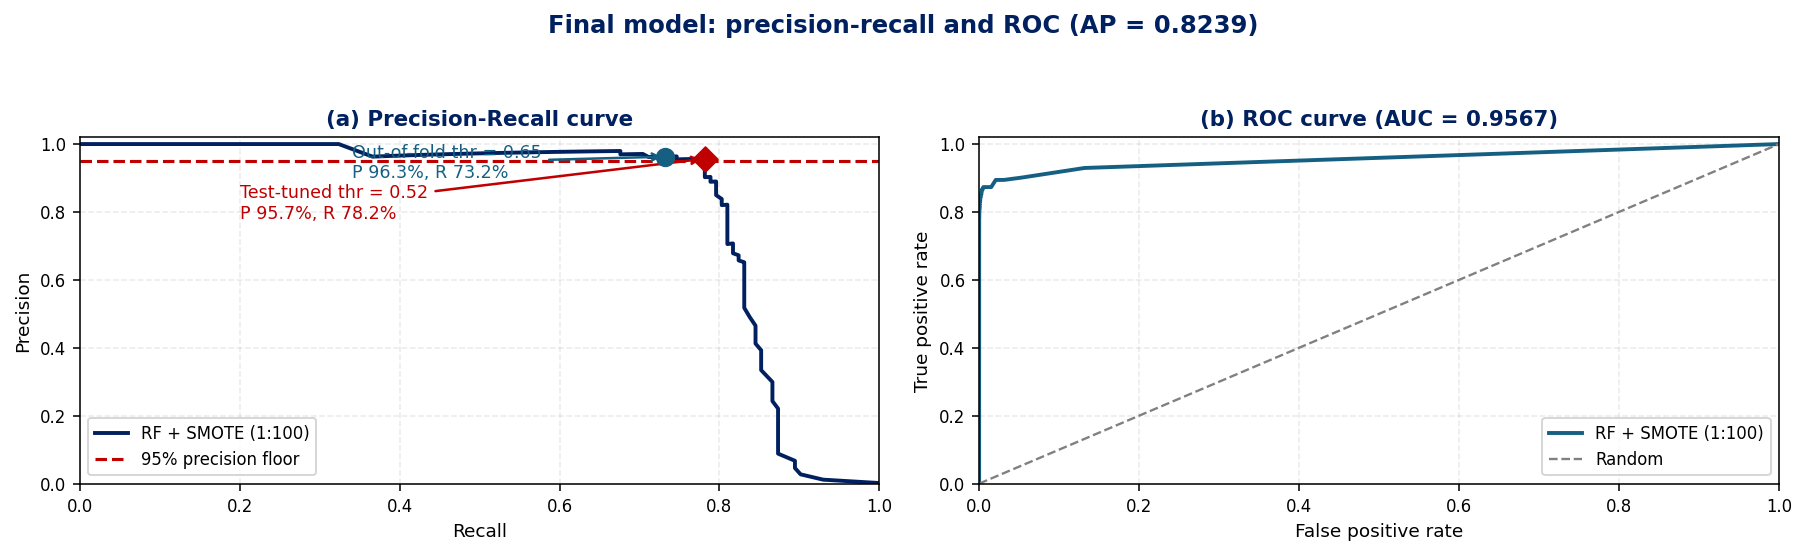
\includegraphics[width=0.95\textwidth]{Images/charts/s7_pr_roc_operating_point.png}
\caption{Precision--recall and ROC curves for the final model. Two operating
points are marked on the PR curve: the test-tuned threshold 0.52 (diamond,
95.7\% precision at 78.2\% recall) and the leakage-free out-of-fold threshold
0.65 (circle, 96.3\% precision at 73.2\% recall). The dashed horizontal line
indicates the 95\% precision constraint. The gap between the two markers is the
price of tuning the threshold on the test set (Section~\ref{sec:leakage}).}
\label{fig:prroc}
\end{figure}

\subsection{Imbalance Benchmark: 27 Configurations}

Table~\ref{tab:bench} presents the main benchmark. Three observations dominate.

\paragraph*{SMOTE helps; Random Undersampling destroys.}
Light oversampling raises Random Forest Average Precision from 0.8055 to 0.8239
at the 1:100 ratio, and to 0.8348 at 1:10. Random Undersampling, by contrast,
collapses it to 0.6883 and renders the precision-constrained recall negligible
(0.035--0.092 across models). The mechanism is straightforward: discarding
roughly 95\% of the legitimate class removes exactly the evidence the model
needs to learn a boundary against the majority.

\begin{table}[h!]
\centering
\caption{Results of the imbalance benchmark on the held-out test set
(85{,}118 transactions, 142 frauds). Only configurations reaching the 95\%
precision constraint are shown for the constrained columns; all F1 values are
measured at that same threshold.}
\label{tab:bench}
\scriptsize
\setlength{\tabcolsep}{2.2pt}
\begin{tabular}{p{1.9cm}p{1.7cm}p{0.85cm}rrrrrr}
\toprule
\textbf{Model} & \textbf{Imbalance} & \textbf{Ratio} & \textbf{AUC-PR} & \textbf{AUC-ROC} & \textbf{F1} & \textbf{Recall} & \textbf{Prec.} & \textbf{Cost} \\
\midrule
Random Forest & SMOTE & 1:100 & 0.8239 & 0.9567 & \textbf{0.8605} & \textbf{0.7817} & 0.9569 & \textbf{\$170.45} \\
Random Forest & SMOTE & 1:20 & 0.8336 & \textbf{0.9806} & 0.8471 & 0.7606 & 0.9558 & \$186.80 \\
Random Forest & SMOTE & 1:10 & 0.8348 & 0.9759 & 0.8425 & 0.7535 & 0.9554 & \$192.25 \\
Random Forest & SMOTE & 1:2 & 0.8309 & 0.9751 & 0.8287 & 0.7324 & 0.9541 & \$208.60 \\
Random Forest & none & --- & 0.8055 & 0.9501 & 0.8605 & 0.7817 & 0.9569 & \$170.45 \\
Random Forest & class\_weight & --- & 0.8239 & 0.9594 & 0.8193 & 0.7183 & 0.9533 & \$219.50 \\
XGBoost & SMOTE & 1:20 & 0.8244 & 0.9761 & 0.8425 & 0.7535 & 0.9554 & \$192.25 \\
XGBoost & none & --- & 0.8213 & 0.9717 & 0.8379 & 0.7465 & 0.9550 & \$197.70 \\
Decision Tree & class\_weight & --- & 0.7130 & 0.9003 & 0.7022 & 0.5563 & 0.9518 & \$344.55 \\
Logistic Regression & none & --- & 0.7092 & 0.9627 & 0.2561 & 0.1479 & 0.9545 & \$659.75 \\
\midrule
Isolation Forest & none & --- & 0.1763 & 0.9407 & 0.2877 & --- & --- & --- \\
\bottomrule
\bottomrule
\end{tabular}

\vspace{2pt}
\footnotesize
\textit{Recall} and \textit{Precision} are measured at the threshold
satisfying the 95\% precision constraint; \textit{F1} is measured at that
same threshold, and \textit{Cost} is the total business cost on the test set
there. XGBoost does not accept a \texttt{class\_weight} argument, so its
\texttt{class\_weight} run is identical to its no-resampling run and is
omitted here; \emph{class weighting} was therefore evaluated on Logistic
Regression, Decision Tree and Random Forest only. Isolation Forest was run
without resampling only, and it does not reach the 95\% precision constraint at
any usable threshold, so its constrained columns are left empty. Its F1 of
0.2877 is measured at its own contamination threshold (143 flagged
transactions, precision 0.2867, recall 0.2887), not at a 95\%-precision
threshold; at the default 0.5 threshold the same model flags 3{,}521
transactions to reach 81.7\% recall.
\end{table}

\begin{figure}[h!]
\centering
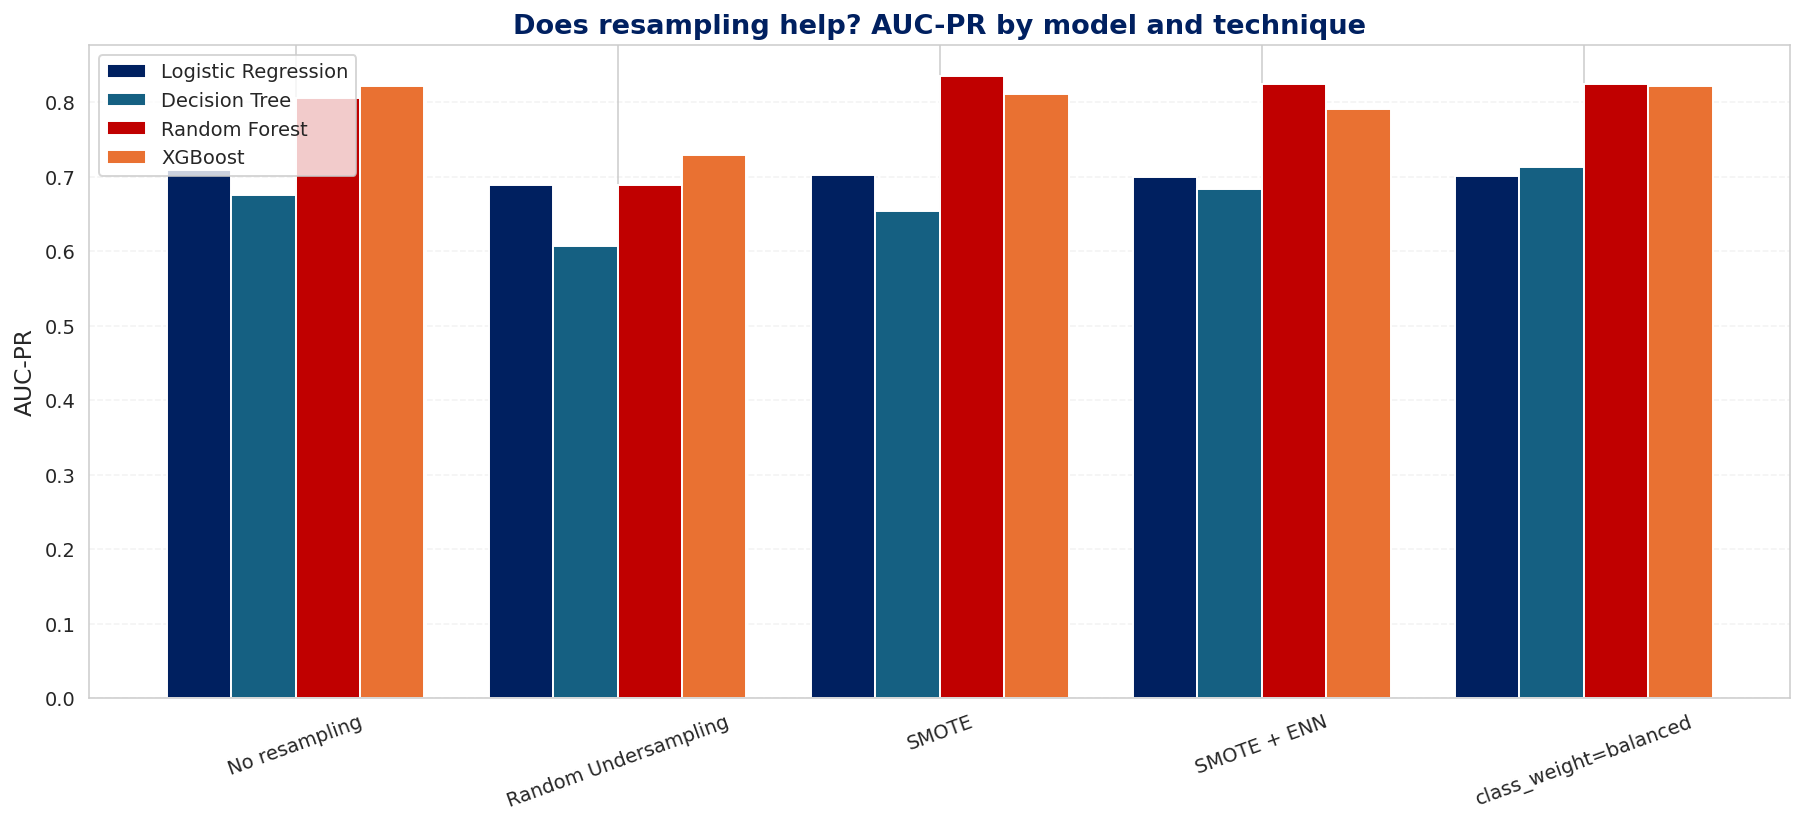
\includegraphics[width=0.70\textwidth]{Images/charts/s5_aucpr_by_technique.png}
\caption{Average Precision by imbalance technique, aggregated over model
families. Random Undersampling lowers Average Precision for every model. SMOTE
and class weighting raise it for the tree ensembles; for Decision Tree,
Logistic Regression and XGBoost the effect of SMOTE is slightly negative
($-0.006$ to $-0.022$).}
\label{fig:aucpr}
\end{figure}

\paragraph*{Logistic Regression fails for reasons unrelated to imbalance.}
Its precision-constrained recall is only 0.1479 --- it catches fewer than one
in six frauds even at a precision of 95\%. Since the same resampling techniques
work well for the tree ensembles on the identical data, the bottleneck is
\emph{model capacity}, not the class ratio. This distinction matters: it shows
that resampling alone cannot substitute for an expressive classifier.

\paragraph*{Unsupervised detection is not operationally viable.}
Isolation Forest attains Average Precision 0.1763 and AUC-ROC 0.9407. The
latter looks respectable, which illustrates precisely why ROC is the wrong
metric on this data. Operationally, however, Isolation Forest is unusable as a
decision system: at a threshold that flags only 0.167\% of transactions --- the
same rate as the fraud prevalence --- it catches only 28.9\% of frauds with a
precision of 28.7\%, and to reach 81.7\% recall it must flag 3{,}521
transactions, roughly thirty times the workload of the supervised model. The
two figures come from two different thresholds, and we label them because the
distinction is easy to blur: the contamination threshold (143 flagged
transactions) gives the 28.9\% recall, while the 3{,}521 figure corresponds to
the default 0.5 score threshold. We note also that this model's threshold is a
quantile of the \emph{test} anomaly scores, so it carries the same
threshold-leakage caveat as the supervised operating points --- the caveat does
not change the conclusion, since the model is unviable by a wide margin either
way. Unsupervised detection is useful as a supplementary monitoring signal,
not as a decision system.

\subsection{Model Selection and the Cost of Over-Searching}
\label{sec:search}

\begin{table}[h!]
\centering
\caption{Effect of expanding the hyper-parameter search. Cross-validated
Average Precision rises slightly while test performance stagnates or degrades.
The CV-AP column is the best cross-validated score found by
\texttt{GridSearchCV} within the grid.}
\label{tab:refine}
\begin{tabular}{p{2.9cm}p{2.6cm}rrrrr}
\toprule
\textbf{Model} & \textbf{Grid} & \textbf{CV-AP} & \textbf{Test AUC-PR} & \textbf{F1@P95} & \textbf{Recall@P95} & \textbf{Time} \\
\midrule
Random Forest & S5 (4 combos) & 0.8536 & \textbf{0.8239} & \textbf{0.8605} & \textbf{0.7817} & 368 s \\
Random Forest & S6 (18 combos) & \textbf{0.8547} & 0.8234 & 0.8605 & 0.7817 & 2{,}448 s \\
XGBoost & S5 (4 combos) & 0.8653 & \textbf{0.8244} & \textbf{0.8425} & \textbf{0.7535} & 19 s \\
XGBoost & S6 (36 combos) & \textbf{0.8689} & 0.8198 & 0.8379 & 0.7465 & 148 s \\
\bottomrule
\end{tabular}
\end{table}

Table~\ref{tab:refine} is an \emph{observation}, not a proof, and we
present it as such. Expanding the grid raised cross-validated Average
Precision by 0.0011 (RF) and 0.0036 (XGBoost) but \emph{lowered} test Average
Precision ($-0.0005$ and $-0.0046$) and reduced precision-constrained recall,
while multiplying training time by up to seven times.

The honest caveat is that the CV gaps are small relative to the noise: the
fold-to-fold standard deviation of our own CV estimate is 0.033--0.045, roughly
thirty times the 0.0011 difference we are discussing, and we ran a single seed.
We therefore do \emph{not} claim to have demonstrated that a wider search
causes overfitting. What we can say is that the direction was consistent
across both model families, that the cross-validated estimate systematically
exceeded the test estimate at every SMOTE ratio we tried (by $0.013$ to
$0.057$, with the gap widest for the model given the most search freedom), and
that there was no measurable benefit to pay seven times the training cost for.
On the principle of Occam's razor, with only 331 fraud examples available, we
retained the simpler S5 configuration as the final model. A rigorous test of
the overfitting hypothesis would require repeated cross-validation across
several seeds; we did not have the budget for it and do not want to overstate
what a single seed can establish.

\subsection{Threshold Selection and Leakage in Threshold Tuning}
\label{sec:leakage}

Selecting an operating threshold on the test set is a subtle form of leakage.
We quantified it by re-deriving the threshold from out-of-fold predictions on
the \emph{training} set only, then applying it unchanged to the test set.

\begin{table}[h!]
\centering
\caption{Effect of the threshold-tuning procedure on measured recall.}
\label{tab:thr}
\begin{tabular}{p{4.6cm}rrrrrr}
\toprule
\textbf{Procedure} & \textbf{Thr.} & \textbf{Prec.} & \textbf{Recall} & \textbf{F1} & \textbf{\#flag} & \textbf{Cost} \\
\midrule
Tuned on test set (optimistic) & 0.5200 & 0.9569 & \textbf{0.7817} & 0.8605 & 116 & \$170.45 \\
Tuned on train (out-of-fold, clean) & 0.6500 & 0.9630 & 0.7324 & 0.8320 & 108 & \$208.30 \\
\midrule
\multicolumn{7}{@{}l}{\footnotesize Difference: $-4.9$ percentage points of recall, $+$USD 37.85 in cost.}\\
\bottomrule
\end{tabular}
\end{table}

The honest recall of our model is therefore \textbf{73.24\%} (leakage-free)
rather than 78.17\% (optimistic). We report both throughout: 78.2\% as the
best-case performance of the operating point, and 73.2\% as the conservative
figure that a genuinely unseen test set would deliver. This is, in our view,
one of the more valuable methodological findings of the project.

\paragraph{What the leakage-free figure does and does not fix.} We report
0.7324 as \emph{more conservative}, but we should be precise about what it
is. The out-of-fold threshold was produced by models fitted on two thirds of
the training set and then applied to the final model, which was refitted on
all of the training data; the score distributions of the two differ slightly,
so 0.7324 is not a perfectly clean holdout estimate either. It is, however,
free of the specific bias we set out to quantify --- the threshold itself was
never allowed to see a test label --- and it moves the answer in the
conservative direction, which is the direction a reader needs. A strictly
correct protocol would reserve a validation split for threshold selection and
never touch it again; we did not, and Section~\ref{sec:discussion} records this
as a limitation of the current work.

\subsection{Explainability}

\begin{figure}[h!]
\centering
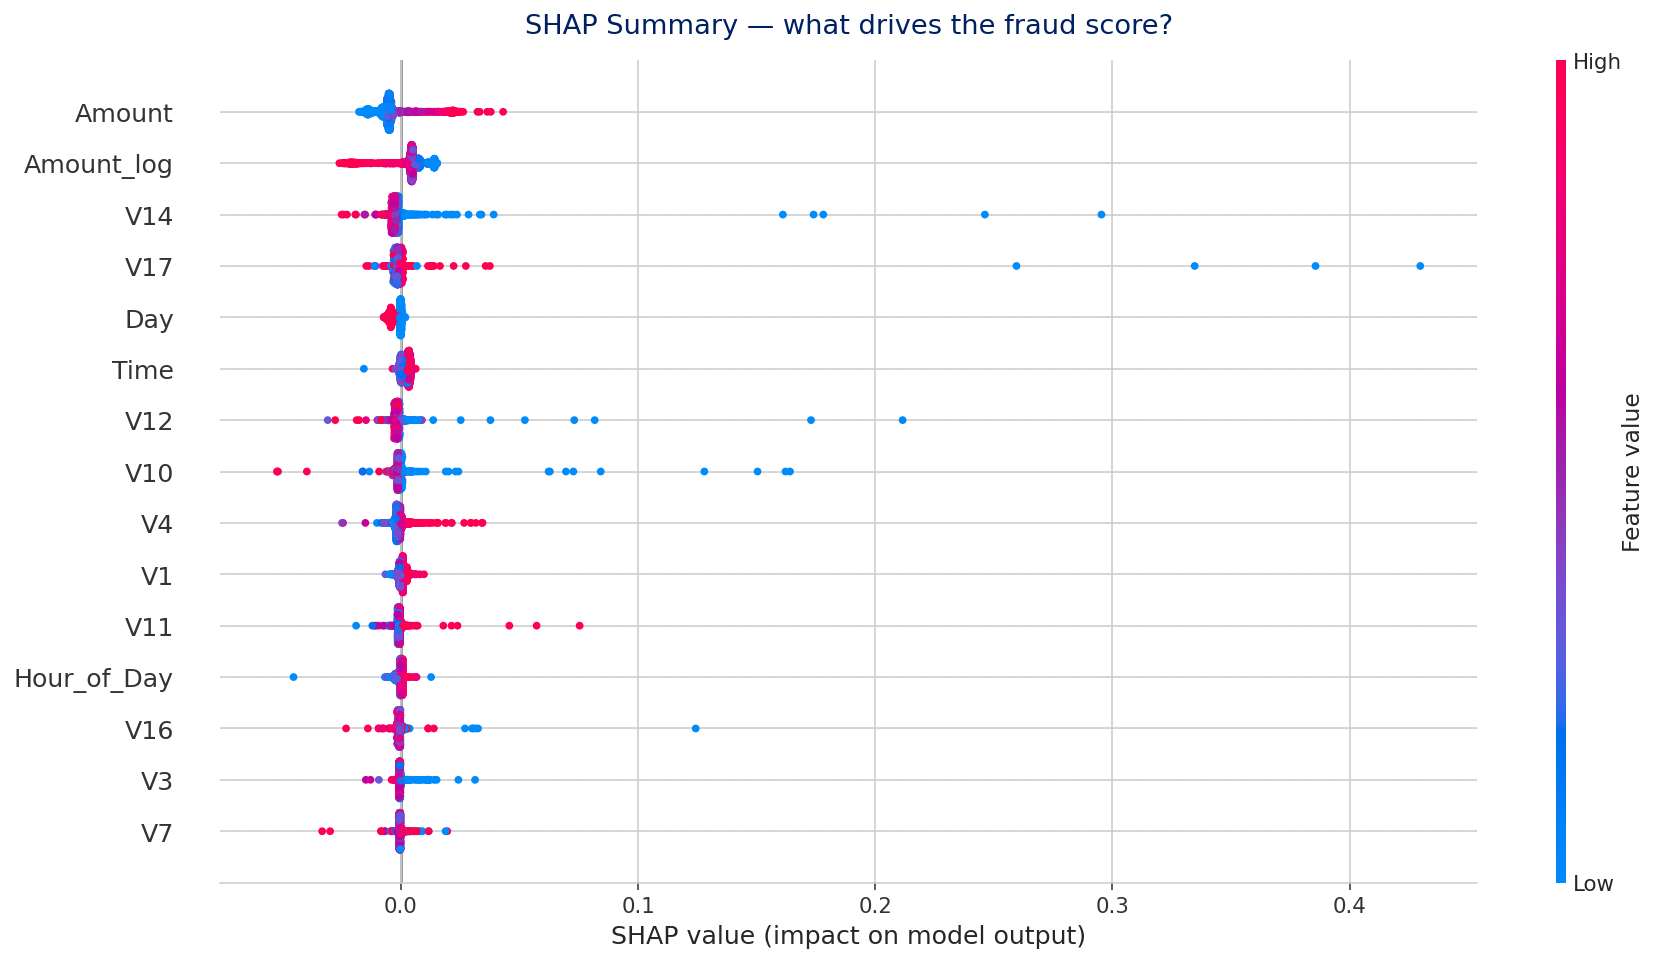
\includegraphics[width=0.78\textwidth]{Images/charts/s8_shap_summary.png}
\caption{SHAP summary (beeswarm) for the fraud class. Each point is one
transaction; horizontal position is the contribution of that feature to the
predicted fraud probability. Amount and Amount\_log dominate, followed by the
PCA components V14 and V17.}
\label{fig:shapsummary}
\end{figure}

We computed both permutation importance on the test set and exact TreeSHAP
values \cite{Lundberg2020}, and verified the additivity property
$\mathrm{base} + \sum_j \phi_j = \hat{p}$ to within $1.8 \times 10^{-13}$,
confirming the implementation is correct.

\paragraph*{Two configurations tie at the operating point, and we say so.}
Random Forest with SMOTE at 1:100 and Random Forest without resampling both
reach recall 0.7817 at USD 170.45 on the test set. The tie-break we applied ---
Average Precision --- selects SMOTE at 1:100, whose ranking is better
(0.8239 against 0.8055) even though the operating point is identical. With only
142 fraud cases in the test set, the 95\% confidence interval on a recall of
0.7817 spans roughly 0.71--0.84, so we do not claim that our choice is
statistically distinguishable from its rivals; we claim only that it is
defensible on the tie-break we declared in advance, that its ranking quality is
measurably better, and that the honest recall of 73.24\% applies to both.

\paragraph*{The default importance measure is wrong on this data.}
Table~\ref{tab:imp} shows that Random Forest's built-in impurity importance
ranks \texttt{Amount} only 21st of 35 features, while permutation importance
ranks it 2nd and SHAP ranks it 1st. The two criteria answer different
questions, and on this data they disagree sharply. Impurity importance measures
the \emph{mean decrease in Gini impurity} attributable to the splits chosen on a
feature, weighted by how pure the resulting leaves are. Because 99.83\% of the
transactions are legitimate, the Gini baseline is already close to zero, and the
absolute impurity decrease contributed by \texttt{Amount} --- whose
discriminative power is essentially threshold-like (small amounts are
legitimate) and therefore diffuse across many splits --- is small even though
destroying that feature costs the model a great deal of accuracy. The PCA
components \texttt{V14} and \texttt{V17}, by contrast, produce few, very pure
leaves and therefore dominate the impurity ranking.

Reporting \texttt{feature\_importances\_} alone would have hidden the most
informative feature in the dataset --- and, with it, the fact that the model's
signal is mostly about transaction size, which is exactly the insight a bank
needs to design an amount-gating policy. The Spearman correlation between
permutation importance and SHAP is 0.766, indicating broad agreement between
the two measure-based approaches.

\begin{table}[h!]
\centering
\caption{Feature importance measured three ways, all on the same test set and
the same final model. Spearman correlation between permutation importance and
SHAP: $\rho = 0.766$ ($p = 8.3 \times 10^{-8}$). Impurity ranks are computed
directly from \texttt{feature\_importances\_} of the fitted forest. The table shows
the five highest-ranked features by permutation importance, the seventh-ranked
\texttt{V9}, and three engineered temporal features reported for contrast; the
other 26 of the 35 are omitted for space, and the full ranking is archived in
\texttt{artifacts/tables/s8\_importance\_comparison.csv}.}
\label{tab:imp}
\begin{tabular}{lrrrr}
\toprule
\textbf{Feature} & \textbf{Perm. imp.} & \textbf{Permutation rank} & \textbf{SHAP rank} & \textbf{Impurity rank} \\
\midrule
\texttt{Amount\_log} & 0.0819 & \textbf{1} & 2 & 15 \\
\texttt{Amount} & 0.0801 & 2 & \textbf{1} & 21 \\
\texttt{V14} & 0.0629 & 3 & 3 & \textbf{1} \\
\texttt{V17} & 0.0431 & 5 & 4 & \textbf{2} \\
\texttt{V4} & 0.0551 & 4 & 9 & 8 \\
\texttt{V9} & 0.0392 & 7 & 20 & 9 \\
\texttt{Day} & 0.0099 & 15 & \textbf{5} & 31 \\
\texttt{Hour\_of\_Day} & 0.0104 & 14 & 12 & 26 \\
\texttt{Is\_Night} & 0.0008 & 31 & 29 & 34 \\
\bottomrule
\end{tabular}
\end{table}

Three of the five engineered features enter the top fifteen by permutation
importance, and \texttt{Day} reaches the top five by SHAP, which justifies the
feature-engineering stage. \texttt{Is\_Night} contributes almost nothing (rank
31 of 35) and could be removed with no measurable loss --- we report this
because it is informative about how little some published feature sets matter.

\begin{figure}[h!]
\centering
% The regenerated PNG is a wide 3-panel banner (2427x907 px, ratio 2.68).
% It is inserted with an explicit \scalebox so that the whole picture -- and
% not just the white margin -- stays inside the text block, with a little
% breathing room on the right so it never looks flush against the edge.
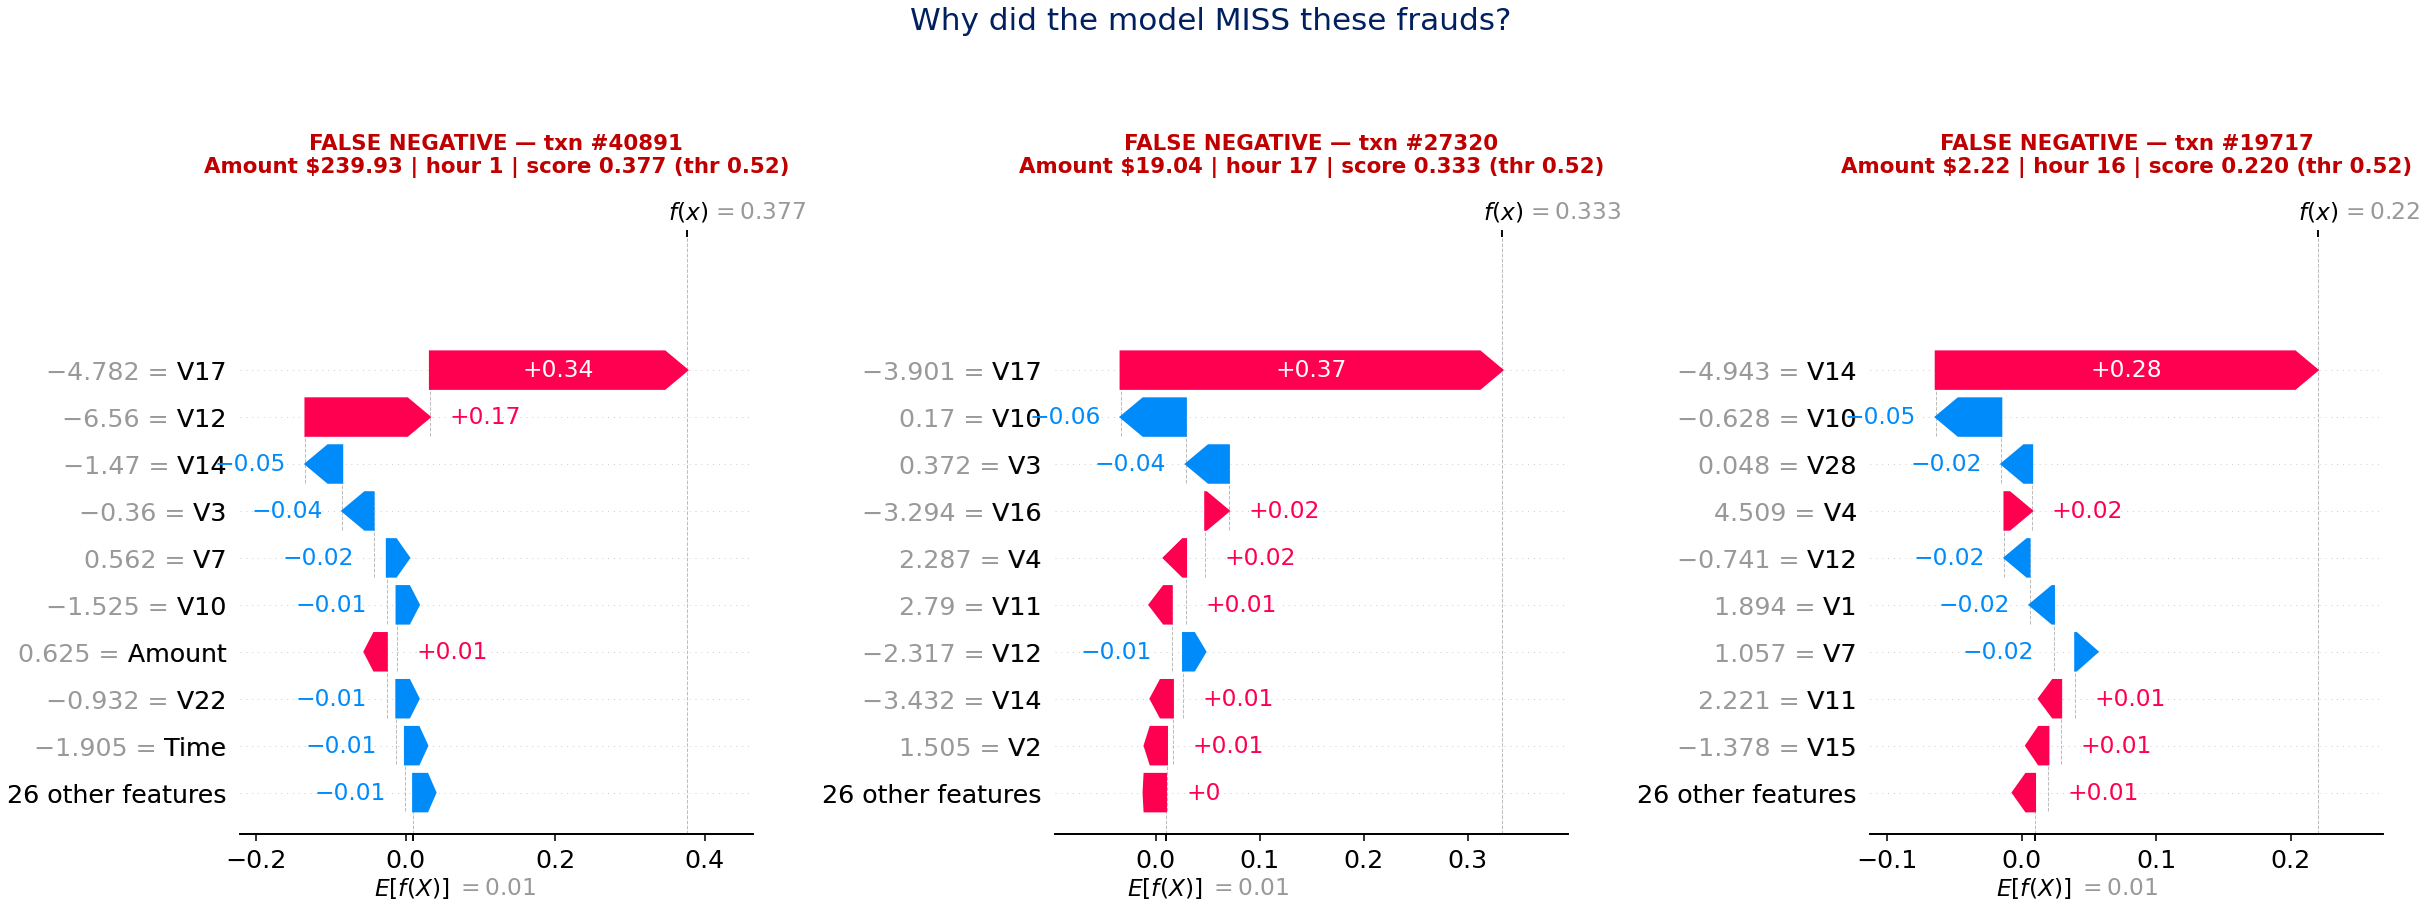
\includegraphics[width=0.80\textwidth, trim=0 0 0 0, clip]{Images/charts/s8_shap_waterfall_fn.png}
\caption{Three false negatives that came closest to detection, explained by
SHAP. Each missed fraud is a low-value transaction made at an unusual hour
(\$239.93 at 01:00, \$19.04 at 17:00, \$2.22 at 16:00).}
\label{fig:waterfallfn}
\end{figure}

\paragraph*{What the model cannot catch.}
Figure~\ref{fig:waterfallfn} explains the 31 missed frauds. Roughly two thirds
of them (64.5\%) have amounts below \$10, and the median missed fraud is USD 3.22 --- \emph{lower}
than the median legitimate transaction of USD 21.90. These transactions are
statistically indistinguishable from ordinary small purchases. Catching them
would require merchant-level, device-fingerprint or behavioural features that
this dataset does not contain.

\subsection{Calibration of the Predicted Probability}

A fraud score is only useful operationally if it can be read as a probability,
because both our cost model and our two-tier policy assume that a score of
0.8 corresponds to an 80\% likelihood of fraud. We verified this empirically.

\begin{figure}[h!]
\centering
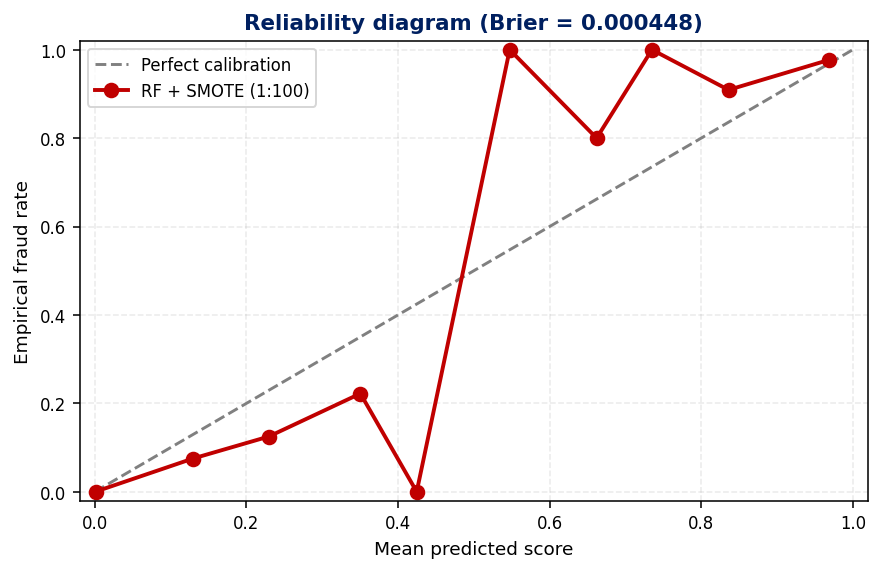
\includegraphics[width=0.55\textwidth]{Images/charts/s10_calibration.png}
\caption{Reliability diagram of the final model. Predicted scores track the
empirical fraud rate closely across the whole range; the Brier score is
0.000448 against a base rate of 0.001668.}
\label{fig:calib}
\end{figure}

The model is well calibrated in the region that matters. In the highest bin
(scores 0.9--1.0, 88 transactions) the mean predicted score is 0.969 and the
empirical fraud rate is 0.977; in the 0.6--0.7 bin the model predicts 0.662
against an empirical 0.800. The overall Brier score of 0.000448 is barely
above the 0.001665 of the trivial always-legitimate predictor, because the
model is nearly always correct when it predicts ``legitimate''. The
reliability diagram in Figure~\ref{fig:calib} shows why this matters: the
score distribution is extremely concentrated --- 99.9\% of all transactions
score below 0.1 --- so the model behaves as a near-perfect ranker with sharp
separation, not as a smoothly calibrated probability surface. It is well
calibrated in the tail that the policy actually uses, which is the only
property the operating policy requires.
